\section{D\'eveloppement logiciel}

\begin{frame}
 	\frametitle{Développement logiciel}
        \tableofcontents[currentsection,hideothersubsections]
\end{frame}

\subsection{Organisation}
\frame
{
\frametitle{Organisation du travail}
\begin{block}{Organisation}
 \begin{itemize}
 \item Travail à distance
 \item Développement itératif
 \end{itemize}
\end{block}

\begin{block}{git}
 \begin{itemize}
  \item Gestionnaire de version
\item Récent 
\item Distribué : machine = client + serveur
\item Performant
 \end{itemize}
\end{block}

}

\subsection{Architecture}
\frame
{
\frametitle{Architecture de la solution propos\'ee}
\framesubtitle{Evolutivité et souplesse}

\begin{minipage}{0.45\textwidth}
\begin{flushleft}
\begin{center}
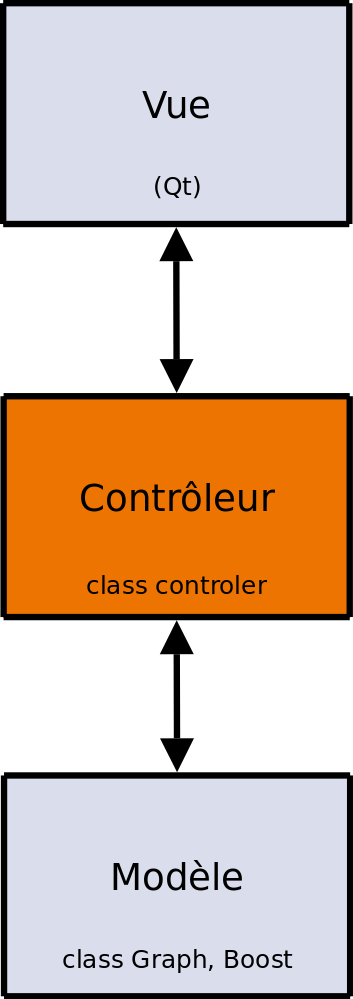
\includegraphics[height=0.95\textheight]{mvcScheme.png}
\end{center}
\end{flushleft}
\end{minipage}
\begin{minipage}{0.45\textwidth}
\begin{flushright}
\begin{block}{Vue}
\begin{center}
Interface graphique de l'utilisateur.
\end{center}
\end{block}
~\\
\begin{block}{Contrôleur}
\begin{center}
Gestion du dialogue entre la partie traitement et l'interface graphique.
\end{center}
\end{block}
~\\
\begin{block}{Modèle}
\begin{center}
Traitement et analyse des données.
\end{center}
\end{block}
\end{flushright}
\end{minipage}
}

\subsection{Boost}
\frame
{
\frametitle{D\'eveloppement avec la librairie Boost}
\begin{block}{Une librairie innovante}
 \begin{itemize}
  \item Utilisation avancée de la généricité...
  \item et de la méta-programmation.
 \end{itemize}
\end{block}

\begin{block}{Difficultés de prise en main}
 \begin{itemize}
  \item Concepts nouveaux
  \item Documentations absconses
  \item \'Eloigné des concepts objets.
 \end{itemize}
\end{block}

}